\subsection{Analysing the results}


\begin{figure}[H]
    \makebox[\textwidth]{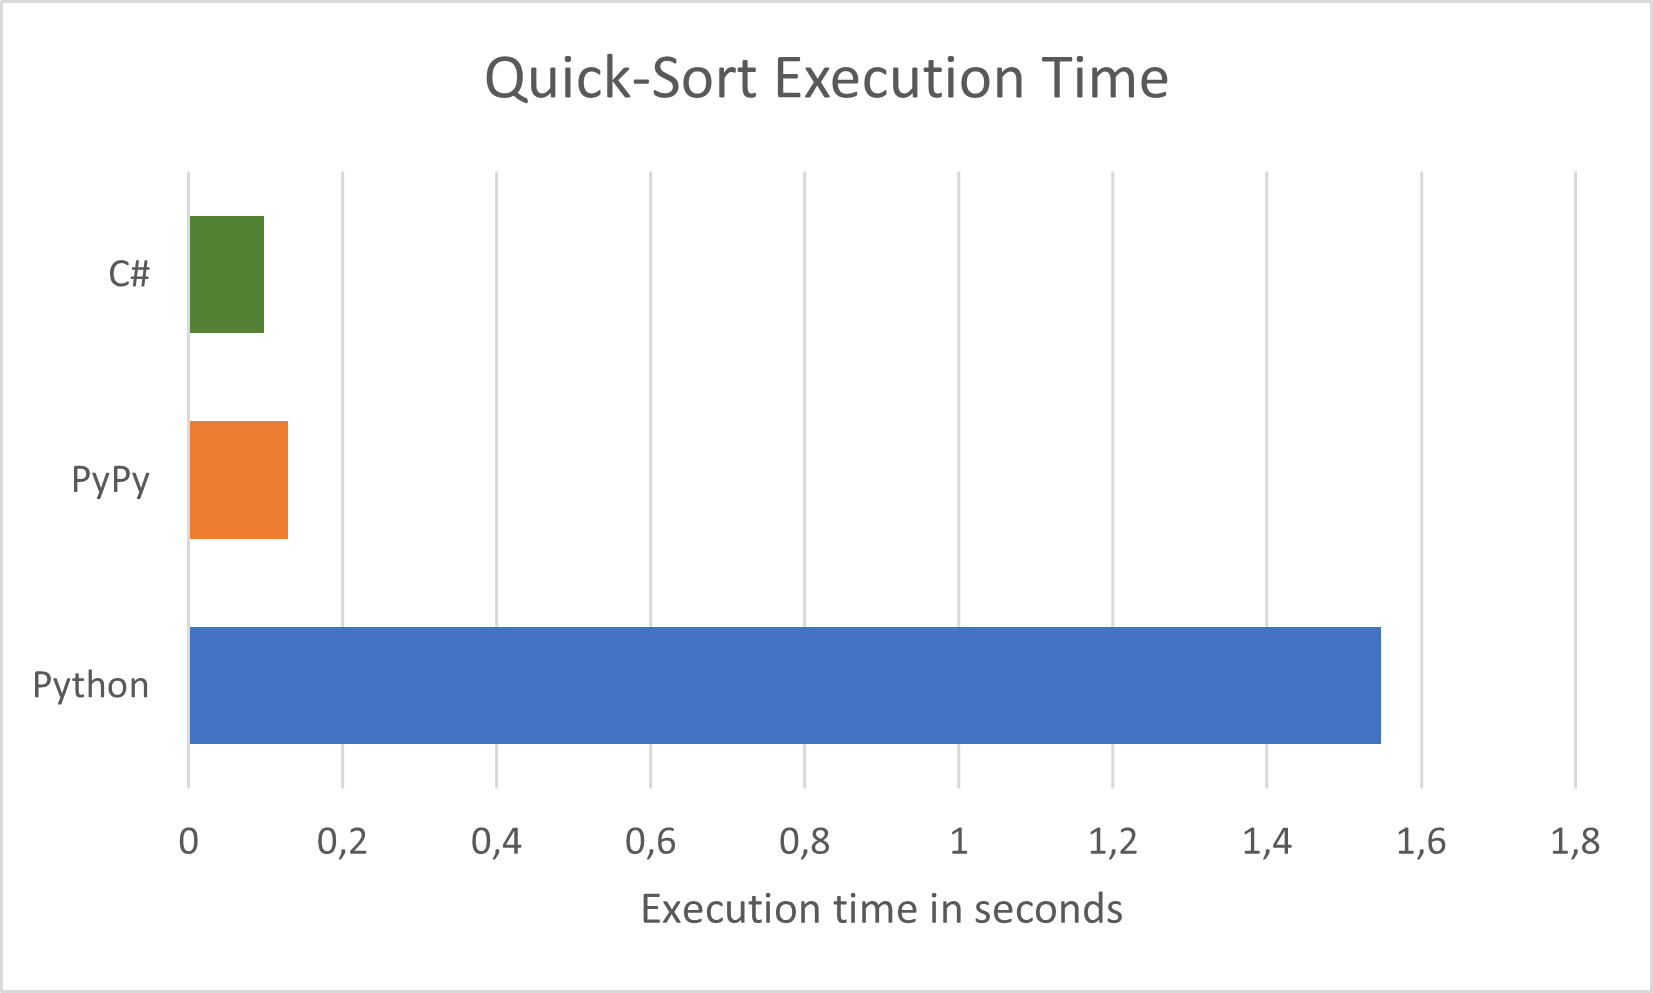
\includegraphics{src/images/qs_time_chart.png}}
    \vspace*{-0.8cm}
    \caption{A column chart that illustrates the difference in execution time}
\end{figure}

In the above diagram you can see the significant difference in execution time. You might wonder why PyPy is not standard if it's so much faster then native Python. The reason for this is that PyPy isn't supported by many of the popular packages, such as Pandas, SciPy and Matplotlib.\cite{quora_pypy}.

\begin{figure}[H]
    \makebox[\textwidth]{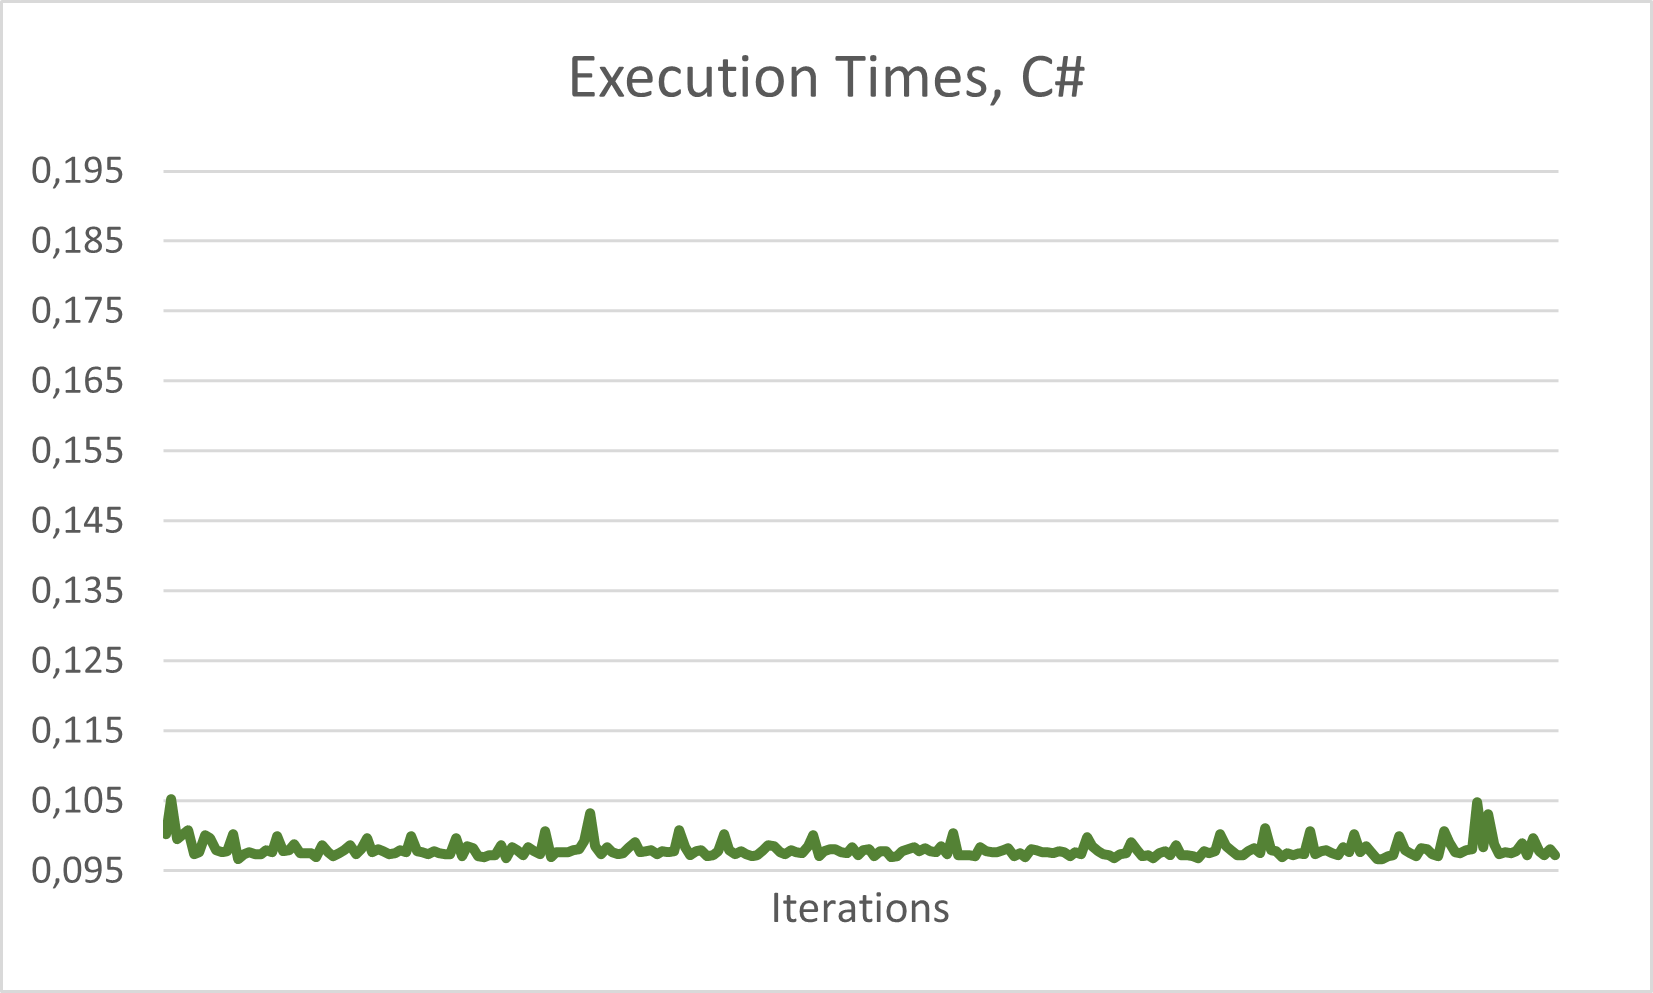
\includegraphics{src/images/qs_exe_time_csharp.png}}
    \vspace*{-0.8cm}
    \caption{A diagram that illustrates the different execution times for each iteration, in C\# for the small text file.}
\end{figure}

\noindent As seen on table \ref{tab:table-comparison_m} in section \ref{sec:results}, the standard deviation for C\# is 0.0011 seconds, which is illustrated in the above line graph, where the execution times spans between 0.105 and 0.095.

\begin{figure}[H]
    \makebox[\textwidth]{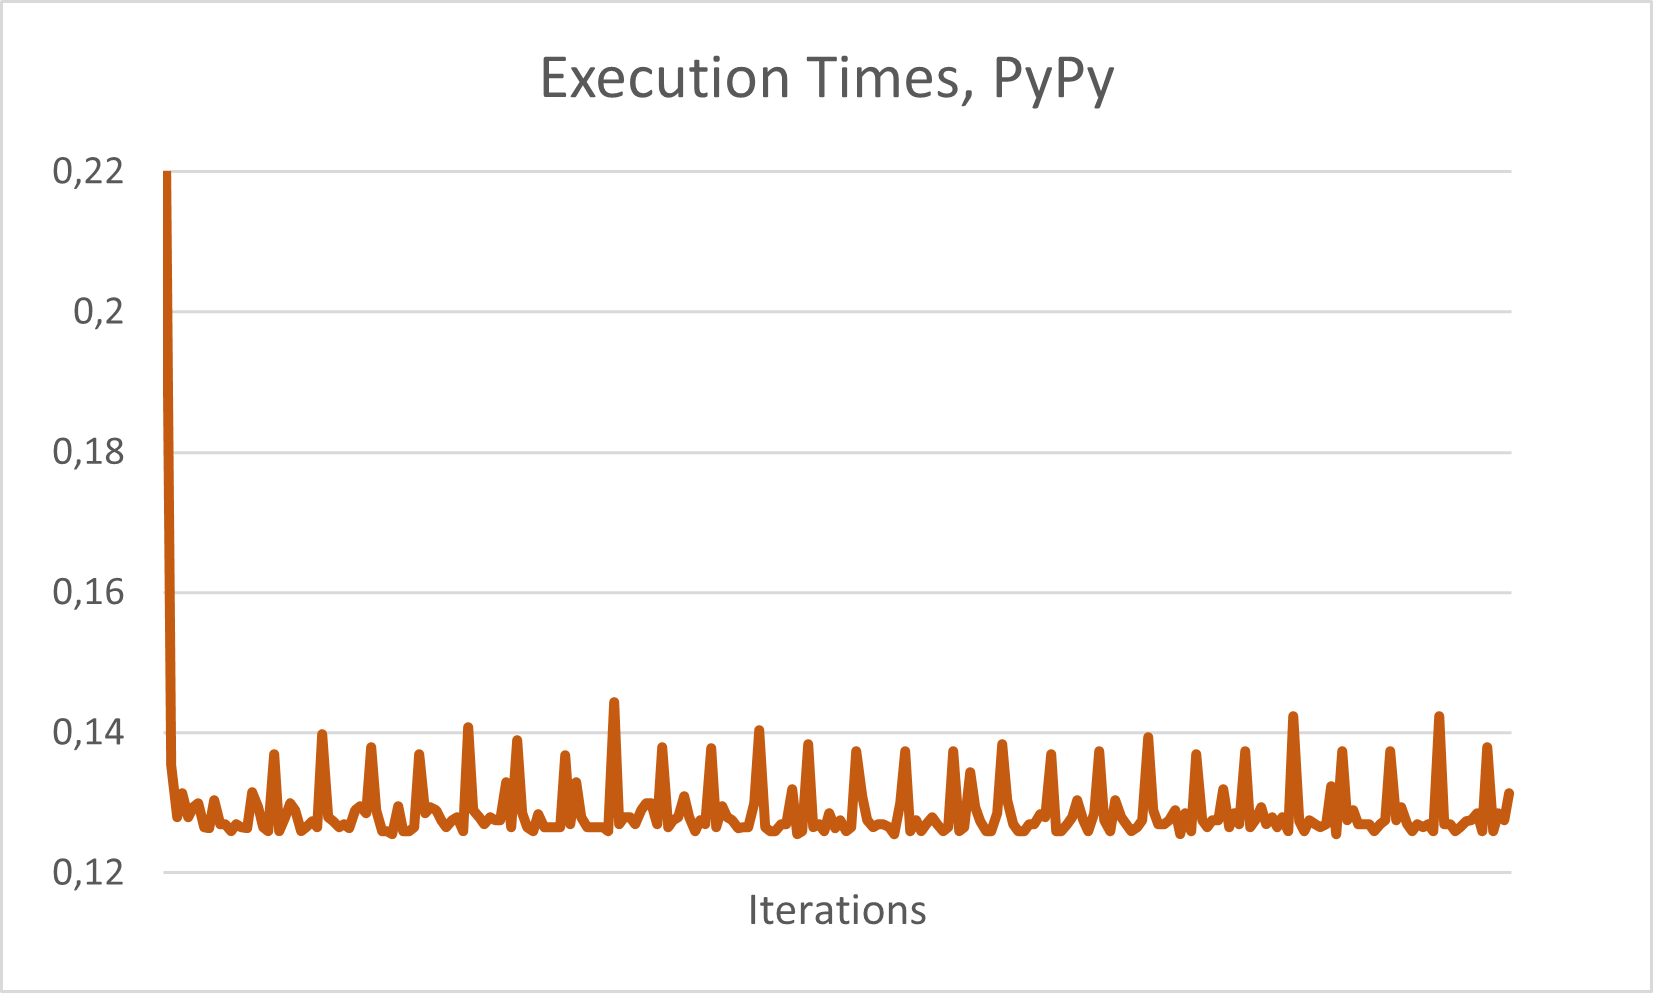
\includegraphics{src/images/qs_exe_time_pypy.png}}
    \vspace*{-0.8cm}
    \caption{A diagram that illustrates the different execution times for each iteration, in PyPY for the small text file.}
\end{figure}

\noindent We can see that the line graph for PyPy looks a lot like the one for C\#. The only difference is the large spike in the beginning. The reason for the spike is that PyPy is both an interpreter and compiler. The first time it runs a program it has to execute it line by line. Where after the JIT compiler comes in to optimize the run time\cite{pypy_org}. 

\begin{figure}[H]
    \makebox[\textwidth]{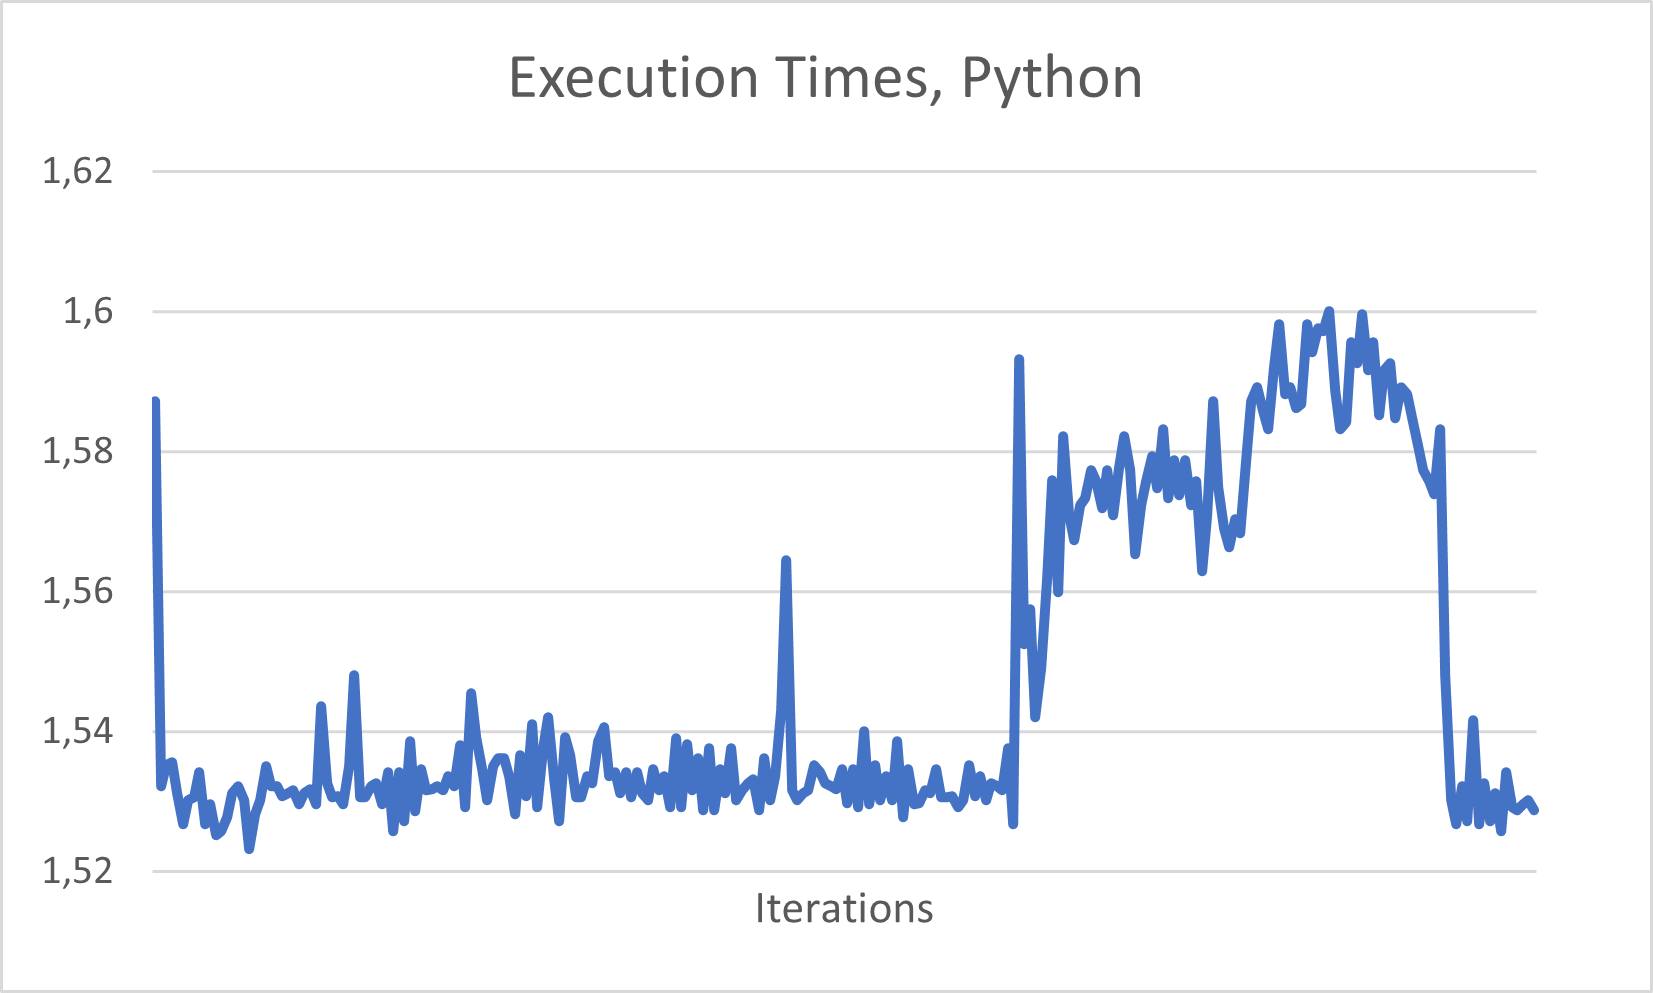
\includegraphics{src/images/qs_exe_time_python.png}}
    \vspace*{-0.8cm}
    \caption{A diagram that illustrates the different execution times for each iteration, in Python for the small text file.}
\end{figure}

\noindent The last group of executions times, are consistent through out my multiple attempts at running the 250 iterations. This proves that it can't be caused by a background program updating. Therefore it either has something to do with my CPU or the way Python handles recursion. 
